\documentclass{llncs}

\usepackage[T1]{fontenc}
\usepackage[utf8]{inputenc}
\usepackage[french]{babel}
\usepackage{graphicx}
\usepackage{amsmath,amssymb}
\usepackage{booktabs}
\usepackage{cite}
\usepackage{siunitx}
\usepackage{xcolor}
\usepackage[hidelinks]{hyperref}

\sisetup{group-digits=none, table-number-alignment=center, output-decimal-marker={,}}
\renewcommand\UrlFont{\color{blue}\rmfamily}
\setlength{\emergencystretch}{1.5em}
\addto\captionsfrench{\renewcommand{\tablename}{Tableau}\renewcommand{\figurename}{Fig.}}
% llncs n'active ses libellés français (« Résumé. », « et »...) qu'avec l'ancien nom babel « frenchb »
\makeatletter
\addto\extrasfrench{\switcht@francais\def\keywordname{{\bfseries Mots-clés\,:}}}
\makeatother

\begin{document}

\title{One-to-one SkewGRAM : appliquer des embeddings du TAL à l'optimisation de graphes biologiques}

\author{Bechir Mady\inst{1} \and
Abderahmane Abderrahmane\inst{1} \and
Mohamedou Yahya Cheikh Mohamed Vall\inst{1} \and
El Moustapha Mohamed El Moustapha\inst{1} \and
Mohamed Lemine Ahmed Sidi\inst{1} \and
Hafedh Mohamed Babou\inst{2}}

\institute{Unité de Recherche en Systèmes Intelligents Avancés (URSIA), Institut Supérieur du Numérique (SupNum), Nouakchott, Mauritanie\\
\email{\{22014,22053,25239,22013\}@supnum.mr, m-lamine.ahmed-sidi@supnum.mr}
\and
École Supérieure Polytechnique (ESP), Nouakchott, Mauritanie\\
\email{hafedh.mohamed-babou@esp.mr}}

\maketitle

\begin{abstract}
Le problème One-to-one SkewGRAM consiste à trouver un plus long chemin dans un graphe orienté acyclique $D$ dont les sommets induisent un sous-graphe connexe dans un graphe non orienté $G$ défini sur le même ensemble de sommets. Il apparaît lorsque l'on compare des voies métaboliques à des réseaux génomiques ou fonctionnels, et il est NP-difficile. Le modèle exact ILP2 demande quelques dizaines de secondes sur des instances de 100 sommets et plusieurs minutes sur des instances de 200 sommets, tandis que les décodeurs à base de réseaux de neurones sur graphes proposés auparavant renvoient des chemins d'environ un sommet. Notre méthode, Skew-GRAM, emprunte le modèle Skip-Gram au traitement automatique des langues (TAL) : les marches aléatoires orientées sur $D$ sont lues comme des phrases, et les embeddings des sommets sont appris avec des exemples négatifs tirés parmi les non-successeurs. Un décodeur Monte-Carlo combine ces embeddings avec une anticipation exacte par programmation dynamique sur $D$ et un bonus pour les sommets adjacents dans $G$ au chemin en construction. Une dernière étape Union-Find extrait le plus long sous-chemin connexe dans $G$, si bien que tout chemin renvoyé est réalisable. Sur 368 instances d'Erd\H{o}s--Rényi disposant d'une solution ILP2, avec cinq graines aléatoires, la méthode atteint la longueur ILP2 dans 71,3\,\% des exécutions à 100 sommets et dans 30,0\,\% à 200 sommets, avec des accélérations médianes par rapport à ILP2 de 4,0$\times$ et 21,2$\times$ ; sur une instance de 200 sommets, elle trouve un chemin plus long que la solution ILP2 fournie. Elle trouve l'optimum exact sur les 25 voies métaboliques KEGG et traite des graphes de 1000 sommets en 143 secondes environ. Sans l'anticipation par programmation dynamique, les chemins sont 23\,\% plus courts sur les instances de 100 sommets.

\keywords{Optimisation combinatoire \and Bio-informatique \and Embeddings de sommets \and Skip-Gram \and Programmation dynamique \and Union-Find.}
\end{abstract}

% ============================================================
\section{Introduction}
% ============================================================

Les systèmes biologiques se décrivent naturellement par des réseaux dont les sommets sont des entités biologiques et dont les arêtes sont des relations entre elles. Comparer deux réseaux construits sur les mêmes entités peut faire apparaître des motifs qu'aucun des deux réseaux ne montre seul. Le métabolisme, par exemple, est un réseau orienté dans lequel les réactions se succèdent le long des voies, tandis que la proximité génomique ou les interactions protéine--protéine donnent un réseau non orienté d'associations fonctionnelles~\cite{sharan2006,zaharia}. Une chaîne de réactions dont les gènes sont aussi proches les uns des autres sur le génome est candidate pour être une unité fonctionnelle conservée.

Le problème \emph{One-to-one SkewGRAM} formalise cette recherche~\cite{fertin2012,sidi2022}. Étant donnés un graphe orienté acyclique $D$ et un graphe non orienté $G$ sur le même ensemble de sommets, il s'agit de trouver un plus long chemin orienté de $D$ dont les sommets induisent un sous-graphe connexe de $G$. Le problème est NP-difficile~\cite{fertin2012,sidi}. Sa difficulté vient de l'interaction entre les deux contraintes : un successeur valide dans $D$ peut rompre la connexité dans $G$, et des sommets proches dans $G$ ne se trouvent pas forcément sur un même chemin de $D$.

Les méthodes exactes résolvent le problème à l'optimum. Le programme linéaire en nombres entiers ILP2~\cite{sidi2022,sidi} demande environ 30 secondes sur les instances de 100 sommets et environ quatre minutes sur les instances de 200 sommets de notre jeu de test. Des approches par apprentissage ont aussi été étudiées~\cite{sidi_dl} : un double réseau convolutif sur graphes suivi d'un post-traitement heuristique, et un encodeur de graphe associé à un décodeur LSTM avec attention (DL2). Leur décodage séquentiel produit des chemins très courts, de 1,2 sommet en moyenne pour DL2.

Cet article suit une autre voie, du traitement automatique des langues (TAL) vers la biologie. Notre méthode, Skew-GRAM, lit les marches aléatoires orientées sur $D$ comme des phrases et apprend des embeddings des sommets avec le modèle Skip-Gram~\cite{mikolov}, comme le font DeepWalk et node2vec pour les graphes~\cite{perozzi,grover}. Les embeddings seuls ne résolvent pas le problème d'optimisation : nous les utilisons comme l'un des trois signaux d'un décodeur conçu pour le problème, à côté d'une anticipation exacte par programmation dynamique sur $D$ et d'un signal de connexité souple issu de $G$. Une étape d'extraction exacte impose ensuite la contrainte de connexité.

Nos contributions sont les suivantes :
\begin{enumerate}
\item un modèle d'embeddings Skip-Gram pour les sommets d'un DAG, entraîné sur des marches aléatoires orientées, avec sous-échantillonnage des hubs et échantillonnage négatif structurel ;
\item un décodeur guidé qui combine une anticipation exacte du plus long chemin dans $D$, la similarité des embeddings et un bonus de connexité dans $G$, suivi d'une extraction exacte par Union-Find qui garantit la réalisabilité ;
\item une évaluation sur 375 instances synthétiques de 100 et 200 sommets (dont 368 avec une solution ILP2) avec cinq graines aléatoires, sur 15 instances plus grandes de 500 et 1000 sommets et sur 25 voies métaboliques réelles de KEGG~\cite{kanehisa2000} dont l'optimum exact est connu, ainsi qu'une ablation de l'anticipation.
\end{enumerate}

% ============================================================
\section{Travaux connexes}
% ============================================================

Le problème One-to-one SkewGRAM appartient à une famille de problèmes de comparaison de réseaux biologiques hétérogènes, comme la recherche de motifs métaboliques et génomiques dans CoMetGeNe~\cite{zaharia} et les méthodes de comparaison de réseaux présentées dans~\cite{sharan2006}. Fertin et al.~\cite{fertin2012} ont étudié sa complexité et proposé des algorithmes exacts. Ahmed Sidi et al.\ ont proposé les programmes linéaires en nombres entiers ILP1 et ILP2~\cite{sidi2022} puis des modèles de programmation par contraintes~\cite{sidi} ; ILP2 est la référence exacte utilisée dans cet article.

Parmi les méthodes d'apprentissage pour l'optimisation combinatoire sur graphes figurent les réseaux de pointeurs~\cite{vinyals2015}, l'apprentissage par renforcement de politiques de construction~\cite{bello2016,dai2017} et l'entraînement non supervisé de réseaux de neurones sur graphes~\cite{karalias2020}. Ces modèles sont entraînés sur de nombreuses instances, puis décodent une solution. Les approches d'apprentissage profond de~\cite{sidi_dl} suivent ce schéma pour notre problème. Notre modèle est au contraire entraîné sur chaque instance séparément, car les identifiants des sommets n'ont pas de sens commun d'un graphe généré indépendamment à l'autre, et les embeddings appris ne font que guider une recherche dont la réalisabilité est garantie de façon exacte. Le modèle d'embeddings lui-même suit word2vec~\cite{mikolov} et ses déclinaisons pour les graphes, DeepWalk~\cite{perozzi} et node2vec~\cite{grover}.

% ============================================================
\section{Formulation du problème}
% ============================================================

Soit $V$ un ensemble de $n$ entités biologiques, $D=(V,A)$ un graphe orienté acyclique qui modélise une relation causale ou séquentielle, et $G=(V,E)$ un graphe non orienté qui modélise une association fonctionnelle. Un chemin $P=(p_1,\ldots,p_k)$ est dit \emph{$(D,G)$-consistant} si
\begin{equation}
(p_i,p_{i+1})\in A \quad (i=1,\ldots,k-1) \qquad\text{et}\qquad G[\{p_1,\ldots,p_k\}] \text{ est connexe}.
\end{equation}
L'objectif est de trouver un chemin $(D,G)$-consistant ayant le plus grand nombre de sommets. La figure~\ref{fig:problem} montre une petite instance.

\begin{figure}[t]
\centering
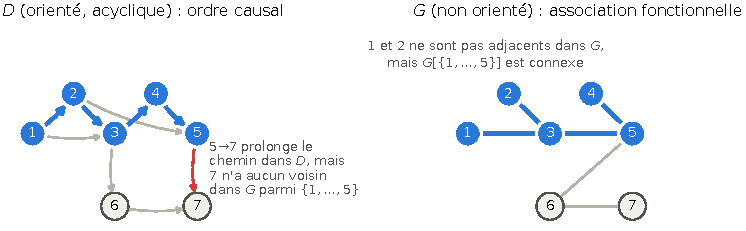
\includegraphics[width=\textwidth]{fig1_problem.pdf}
\caption{Instance jouet à sept sommets. Le chemin mis en évidence $1\to2\to3\to4\to5$ est l'unique optimum. Le prolonger par l'arc $5\to7$ donne le plus long chemin de $D$, mais le sommet 7 n'a aucun voisin dans $G$ parmi les autres sommets du chemin. Le préfixe $(1,2)$ n'est pas connexe dans $G$, alors que le chemin complet l'est.}
\label{fig:problem}
\end{figure}

\subsubsection{La connexité ne peut pas être vérifiée de façon incrémentale.}
\label{sec:incremental}
La contrainte de connexité est globale. Deux sommets consécutifs d'un chemin réalisable ne sont pas forcément adjacents dans $G$, et un préfixe d'un chemin réalisable peut être non connexe dans $G$ alors que le chemin complet l'est (figure~\ref{fig:problem}). C'est le cas général : dans notre jeu de test, les 368 solutions ILP2 contiennent toutes deux sommets consécutifs non adjacents dans $G$, et 363 d'entre elles (98,6\,\%) ont un préfixe non connexe. Un décodeur qui rejetterait toute extension rendant le préfixe courant non connexe ne pourrait construire la plupart de ces solutions. Notre décodeur n'utilise donc $G$ que comme un signal souple pendant la construction du chemin, et vérifie la connexité de façon exacte une fois le chemin terminé.

% ============================================================
\section{Méthode}
\label{sec:method}
% ============================================================

Skew-GRAM comprend un encodeur, qui apprend les embeddings des sommets à partir de $D$ seulement, et un décodeur, qui construit des chemins à partir de $D$, des embeddings et de $G$ (figure~\ref{fig:pipeline}). La méthode s'exécute une fois par instance, en quatre phases. L'analogie qui la guide vient du TAL : un sommet joue le rôle d'un mot, une marche aléatoire orientée celui d'une phrase, et le voisinage d'un sommet dans une marche celui de son contexte.

\begin{figure}[t]
\centering
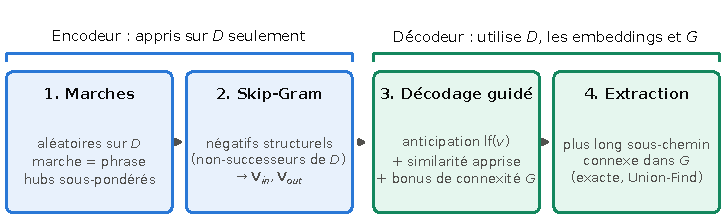
\includegraphics[width=\textwidth]{fig2_pipeline.pdf}
\caption{Les quatre phases de Skew-GRAM, exécutées une fois par instance. L'encodeur apprend les embeddings $\mathbf{V}_{in},\mathbf{V}_{out}$ à partir des marches sur $D$ ; le décodeur génère des chemins candidats (étape~A) et extrait de chacun un sous-chemin $(D,G)$-consistant (étape~B).}
\label{fig:pipeline}
\end{figure}

\subsubsection{Phase 1 : marches aléatoires et sous-échantillonnage des hubs.}
Depuis chaque sommet ayant au moins un successeur, nous lançons plusieurs marches aléatoires qui suivent les arcs sortants de $D$ : depuis le sommet $u$, le sommet suivant est tiré uniformément parmi ses successeurs $N^+(u)$. Une marche s'arrête sur un puits ou à une longueur maximale. Comme dans word2vec, chaque occurrence d'un sommet $v$ de fréquence relative $f(v)$ est conservée avec la probabilité $\min\bigl(1,\sqrt{t/f(v)}+t/f(v)\bigr)$, $t=10^{-3}$, ce qui réduit le poids des hubs. Une fenêtre glissante sur chaque marche produit ensuite les couples (centre, contexte).

\subsubsection{Phase 2 : embeddings Skip-Gram avec négatifs structurels.}
Nous apprenons deux matrices $\mathbf{V}_{in},\mathbf{V}_{out}\in\mathbb{R}^{n\times d}$. Pour un sommet central $c$, un sommet de contexte $o$ et $K$ sommets négatifs $n_1,\ldots,n_K$, la perte est l'objectif classique d'échantillonnage négatif
\begin{equation}
\mathcal{L}(c,o,n_{1:K}) = -\log\sigma(\mathbf{v}_{in,c}^{\top}\mathbf{v}_{out,o}) - \sum_{k=1}^{K}\log\sigma(-\mathbf{v}_{in,c}^{\top}\mathbf{v}_{out,n_k}).
\end{equation}
La différence avec le Skip-Gram standard tient à la façon de tirer les négatifs : au lieu d'une distribution fondée sur les fréquences, les négatifs de $c$ sont tirés uniformément parmi les sommets qui ne sont pas des successeurs de $c$ dans $D$. Le signal négatif reflète ainsi l'orientation des arcs. Le décodeur utilise la similarité $\operatorname{sim}(u,v)=\mathbf{v}_{in,u}^{\top}\mathbf{v}_{out,v}$.

\subsubsection{Phase 3 : décodage guidé (étape A).}
Un décodeur guidé par la seule similarité tend à choisir des successeurs qui mènent rapidement à un puits. Nous calculons donc, pour chaque sommet $v$, le nombre $\mathrm{lf}(v)$ d'arcs d'un plus long chemin de $D$ partant de $v$ :
\begin{equation}
\mathrm{lf}(v) = 0 \ \text{si } N^+(v)=\emptyset, \qquad \mathrm{lf}(v)=\max_{w\in N^+(v)}\bigl(1+\mathrm{lf}(w)\bigr) \ \text{sinon}.
\end{equation}
Comme $D$ est acyclique, toutes les valeurs s'obtiennent en un seul parcours d'un ordre topologique inversé, en temps $O(|V|+|A|)$~\cite{bellman1958}. Lorsque le sommet courant est $u$ et que $v\in N^+(u)$ n'a pas encore été visité, le décodeur attribue à $v$ le score
\begin{equation}
S(u,v) = \frac{\mathrm{lf}(v)}{\tau_{lf}} + \beta\,\frac{\operatorname{sim}(u,v)}{\tau} + \log(\gamma)\,\mathbb{I}_G(v),
\end{equation}
où $\mathbb{I}_G(v)=1$ si $v$ est adjacent dans $G$ à un sommet du chemin en construction, et $0$ sinon. Le sommet suivant est tiré avec la probabilité $P(v\mid u)\propto\exp S(u,v)$. Les trois termes mesurent respectivement le potentiel de chemin restant dans $D$, la compatibilité apprise entre $u$ et $v$, et une préférence pour les sommets reliés dans $G$ au chemin déjà construit. Les sommets visités sont masqués. Le décodeur répète $W$ fois ces marches depuis des sommets de départ tirés uniformément.

\subsubsection{Phase 4 : extraction exacte (étape B).}
Un chemin candidat $P=(p_1,\ldots,p_L)$ issu de la phase~3 est un chemin de $D$, mais il peut ne pas être connexe dans $G$. Tout sous-chemin contigu de $P$ reste un chemin de $D$ ; il suffit donc de trouver le plus long intervalle $[i,j]$ tel que $G[\{p_i,\ldots,p_j\}]$ soit connexe. Pour chaque début $i$, nous étendons la fenêtre d'un sommet à la fois et maintenons les composantes de la fenêtre dans une structure Union-Find~\cite{tarjan1975}, en comparant chaque nouveau sommet aux sommets déjà présents dans la fenêtre. Le coût est en $O(L^3\alpha(L))$ pour un chemin de longueur $L$, où $\alpha$ est la réciproque de la fonction d'Ackermann. L'extraction n'est lancée que lorsque le candidat brut est plus long que le meilleur sous-chemin trouvé jusque-là, et $L$ est borné par le plus long chemin de $D$ (au plus 100 sommets dans nos instances). Le meilleur sous-chemin extrait sur les $W$ marches est renvoyé ; il est $(D,G)$-consistant par construction.

% ============================================================
\section{Expériences}
% ============================================================

\subsection{Protocole expérimental}

\subsubsection{Instances synthétiques.}
Le jeu de test principal contient 300 instances de $n=100$ sommets et 75 instances de $n=200$ sommets, chacune fournie avec la solution d'ILP2 (chemin et temps de calcul). $D$ est construit en tirant un ordre topologique aléatoire puis en ajoutant chaque arc « vers l'avant » avec la probabilité $p$ ($p=0{,}08$ pour $n=100$, $p=0{,}05$ pour $n=200$), et $G$ est un graphe d'Erd\H{o}s--Rényi $G(n,p)$ indépendant~\cite{erdos1959}. ILP2 ne renvoie aucune solution pour 2 instances de 100 sommets et 5 instances de 200 sommets ; elles sont exclues de toutes les comparaisons avec ILP2, ce qui laisse 298 et 70 instances. ILP2 est un modèle exact, mais les solutions fournies ne sont pas toutes optimales : sur l'instance 200\_68, Skew-GRAM trouve un chemin réalisable de 10 sommets, que nous avons vérifié de façon indépendante, alors que le fichier ILP2 en indique 7. Nous utilisons donc les solutions ILP2 comme longueurs de référence, et nous disons qu'une exécution atteint ILP2 lorsque son chemin est au moins aussi long. Pour étudier le passage à l'échelle, nous utilisons aussi 10 instances de $n=500$ sommets et 5 instances de $n=1000$ sommets, construites de la même manière avec $p=0{,}05$ (nous avons généré nous-mêmes les instances de 1000 sommets) ; aucune solution ILP2 n'est disponible pour elles.

\subsubsection{Réseaux métaboliques réels.}
Nous utilisons 25 voies métaboliques de KEGG~\cite{kanehisa2000}, issues de sept bactéries (codes KEGG aae, bsu, eco, mtv, pae, sau et syn). Dans chaque instance, $D$ est le graphe métabolique d'une voie et $G$ un graphe de proximité génomique ou fonctionnelle sur les mêmes sommets. L'ensemble contient 19 voies acycliques (au plus trois par organisme, avec 10 à 80 entités listées) et 6 voies dont les seuls cycles sont des réactions réversibles (2-cycles) ; les sommets sans aucun arc ni arête sont écartés au chargement, ce qui laisse de 4 à 38 sommets. Chaque réaction réversible est orientée de l'identifiant de sommet le plus petit vers le plus grand afin que $D$ soit acyclique ; il s'agit d'une simplification de modélisation. Ces instances n'ont pas de solution ILP2, mais elles sont petites : nous calculons donc leur optimum exact en énumérant les chemins de $D$ avec deux coupes exactes. Les sommets d'un chemin réalisable appartiennent à une même composante connexe $C$ de $G$, si bien que seuls les chemins de $D[C]$ sont énumérés, et un chemin qui se termine en $u$ ne peut gagner plus de $\mathrm{lf}(u)$ sommets.

\subsubsection{Déroulement.}
Le tableau~\ref{tab:hyper} donne les hyperparamètres, identiques pour toutes les instances. L'entraînement utilise Adam~\cite{kingma2014}. Chaque instance est résolue avec cinq graines (42 à 46) ; la graine est réinitialisée au début de chaque instance, si bien qu'un résultat ne dépend pas de l'ordre de traitement des instances. Nous vérifions que chaque chemin renvoyé est $(D,G)$-consistant. Skew-GRAM tourne sur un processeur d'ordinateur portable Intel Core i5-1135G7 (4 c\oe{}urs), avec quatre instances résolues en parallèle sur un fil d'exécution chacune ; le portable servait aussi à d'autres tâches pendant les calculs, si bien que les temps comportent un bruit lié à la charge. Les temps d'ILP2 proviennent des fichiers du jeu de données et ont été mesurés sur une autre machine : les accélérations sont donc seulement indicatives.

\begin{table}[t]
\centering
\caption{Hyperparamètres, identiques pour toutes les instances.}
\label{tab:hyper}
\begin{tabular}{@{}llr@{\qquad}llr@{}}
\toprule
\multicolumn{3}{@{}l}{Encodeur (phases 1--2)} & \multicolumn{3}{l@{}}{Décodeur (phases 3--4)} \\
\midrule
Marches par sommet & & 40 & Marches de décodage & $W$ & 30\,000 \\
Longueur max.\ d'une marche & & 30 & Température d'anticipation & $\tau_{lf}$ & 1,5 \\
Fenêtre de contexte & & 3 & Température de similarité & $\tau$ & 0,5 \\
Dimension des embeddings & $d$ & 32 & Poids de la similarité & $\beta$ & 0,3 \\
Négatifs par couple & $K$ & 5 & Bonus de connexité $G$ & $\gamma$ & 6,0 \\
Époques / taux d'appr. & & 8 / 0,01 & & & \\
\bottomrule
\end{tabular}
\end{table}

\subsection{Comparaison avec ILP2}
\label{sec:ilp2}

Le tableau~\ref{tab:results} résume les résultats. Les valeurs après $\pm$ sont les écarts-types, entre les cinq graines, de la moyenne correspondante, sauf pour les temps de calcul, où il s'agit de l'écart-type sur l'ensemble des exécutions.

\begin{table}[t]
\centering
\caption{Skew-GRAM comparé à ILP2 sur les instances synthétiques disposant d'une solution ILP2 (cinq graines par instance). Exécutions atteignant ILP2 : exécutions dont le chemin est au moins aussi long que la solution ILP2. Accélération : médiane, sur les instances, du rapport entre le temps d'ILP2 et le temps moyen de Skew-GRAM.}
\label{tab:results}
% Généré par scripts/make_paper_assets.py — ne pas modifier à la main.
\setlength{\tabcolsep}{7pt}
\begin{tabular}{@{}l S[table-format=-3.2]@{\,$\pm$\,}S[table-format=1.2] S[table-format=-3.2]@{\,$\pm$\,}S[table-format=1.2]@{}}
\toprule
 & \multicolumn{2}{c}{$n=100$} & \multicolumn{2}{c}{$n=200$} \\
\midrule
Instances avec une solution ILP2 & \multicolumn{2}{c}{298 / 300} & \multicolumn{2}{c}{70 / 75} \\
\addlinespace
\emph{ILP2} \\
\quad Longueur moyenne (sommets) & \multicolumn{2}{c}{9{,}93} & \multicolumn{2}{c}{9{,}64} \\
\quad Temps moyen (s) & \multicolumn{2}{c}{29{,}1} & \multicolumn{2}{c}{251{,}8} \\
\addlinespace
\emph{Skew-GRAM} \\
\quad Longueur moyenne (sommets) & 9.47 & 0.02 & 7.89 & 0.12 \\
\quad Écart moyen à ILP2 (\%) & -4.4 & 0.2 & -17.2 & 0.9 \\
\quad Exécutions atteignant ILP2 (\%) & 71.3 & 2.1 & 30.0 & 4.8 \\
\quad Exécutions à 1 sommet au plus (\%) & 90.3 & 1.0 & 53.1 & 3.3 \\
\quad Temps moyen (s) & 6.9 & 2.6 & 11.3 & 4.2 \\
\addlinespace
Accélération médiane / ILP2 & \multicolumn{2}{c}{4{,}0$\times$} & \multicolumn{2}{c}{21{,}2$\times$} \\
\bottomrule
\end{tabular}

\end{table}

À 100 sommets, les chemins trouvés par Skew-GRAM comptent 9,47 sommets en moyenne, contre 9,93 pour ILP2, soit un écart moyen de $-4{,}4$\,\%. La méthode atteint la longueur ILP2 dans 71,3\,\% des exécutions et en reste à au plus un sommet dans 90,3\,\%. Une exécution dure 6,9\,s en moyenne, contre 29,1\,s pour ILP2. À 200 sommets, le problème est plus difficile pour l'heuristique : l'écart moyen passe à $-17{,}2$\,\% et la longueur ILP2 est atteinte dans 30,0\,\% des exécutions. ILP2 ralentit beaucoup plus, de 29,1\,s à 251,8\,s en moyenne, alors que Skew-GRAM passe de 6,9\,s à 11,3\,s : l'accélération médiane passe ainsi de 4,0$\times$ à 21,2$\times$ (figure~\ref{fig:results}b). À 100 sommets, aucune exécution ne renvoie un chemin plus long que celui d'ILP2 ; à 200 sommets, c'est le cas de quatre exécutions sur cinq pour l'instance 200\_68 (tableau~\ref{tab:instances}). Pour mémoire, DL2~\cite{sidi_dl} trouvait des chemins de 1,2 sommet en moyenne sur des instances de 50 sommets ; nous ne l'avons pas relancé, ce chiffre n'est donc qu'indicatif.

\begin{figure}[t]
\centering
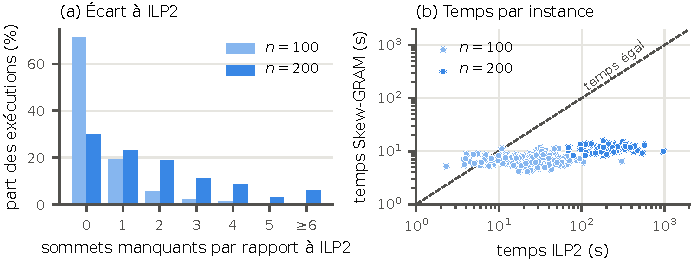
\includegraphics[width=\textwidth]{fig3_results.pdf}
\caption{(a) Nombre de sommets manquant au chemin de Skew-GRAM par rapport à la solution ILP2, sur l'ensemble des exécutions (0 : longueur ILP2 atteinte ou dépassée). (b) Temps de calcul par instance (Skew-GRAM : moyenne sur les cinq graines) ; les points sous la droite en pointillés sont plus rapides avec Skew-GRAM.}
\label{fig:results}
\end{figure}

Le tableau~\ref{tab:instances} détaille dix instances, choisies aux 0\textsuperscript{e}, 50\textsuperscript{e}, 80\textsuperscript{e}, 95\textsuperscript{e} et 100\textsuperscript{e} centiles de l'écart moyen pour chaque taille. À 100 sommets, la plupart des instances atteignent la longueur ILP2, et l'écart se concentre sur quelques instances pour lesquelles les marches guidées atteignent rarement la région de $D$ qui contient le meilleur chemin. À 200 sommets, les écarts sont plus grands (jusqu'à 8 sommets pour une exécution), tandis que sur l'instance 200\_68 Skew-GRAM dépasse la solution ILP2 dans quatre exécutions sur cinq.

\begin{table}[t]
\centering
\caption{Résultats par instance pour dix instances, choisies aux 0\textsuperscript{e}, 50\textsuperscript{e}, 80\textsuperscript{e}, 95\textsuperscript{e} et 100\textsuperscript{e} centiles de l'écart moyen pour chaque taille (de la meilleure à la moins bonne). Skew-GRAM : moyenne $\pm$ écart-type sur les cinq graines. Un écart positif signifie un chemin plus long que la solution ILP2.}
\label{tab:instances}
% Généré par scripts/make_paper_assets.py — ne pas modifier à la main.
\setlength{\tabcolsep}{7pt}
\begin{tabular}{@{}l S[table-format=2.0] S[table-format=2.1]@{\,$\pm$\,}S[table-format=1.1] S[table-format=-2.1] S[table-format=3.1] S[table-format=2.1]@{}}
\toprule
 & \multicolumn{3}{c}{Longueur (sommets)} & {Écart} & \multicolumn{2}{c}{Temps (s)} \\
\cmidrule(lr){2-4} \cmidrule(l){6-7}
{Instance} & {ILP2} & \multicolumn{2}{c}{Skew-GRAM} & {(\%)} & {ILP2} & {Skew-GRAM} \\
\midrule
100\_4 & 11 & 11.0 & 0.0 & 0.0 & 29.0 & 6.1 \\
100\_230 & 10 & 9.8 & 0.4 & -2.0 & 16.1 & 8.2 \\
100\_133 & 13 & 12.0 & 0.0 & -7.7 & 20.6 & 6.4 \\
100\_247 & 6 & 5.0 & 0.0 & -16.7 & 27.0 & 9.3 \\
100\_300 & 9 & 5.0 & 0.0 & -44.4 & 16.9 & 7.9 \\
\addlinespace
200\_68 & 7 & 9.2 & 1.3 & 31.4 & 183.9 & 11.9 \\
200\_50 & 9 & 7.6 & 1.3 & -15.6 & 134.6 & 9.1 \\
200\_61 & 7 & 5.0 & 0.0 & -28.6 & 440.3 & 12.5 \\
200\_49 & 9 & 5.4 & 0.9 & -40.0 & 225.2 & 11.2 \\
200\_41 & 13 & 7.2 & 1.6 & -44.6 & 108.1 & 12.4 \\
\bottomrule
\end{tabular}

\end{table}

\subsubsection{Stabilité selon la graine.}
Le décodeur est stochastique ; nous mesurons donc la variation des résultats selon la graine. La longueur moyenne sur l'ensemble des instances est très stable (écart-type de 0,02 sommet pour $n=100$ et de 0,12 pour $n=200$). Au niveau de chaque instance, la longueur renvoyée varie avec la graine de 0,43 sommet en moyenne (écart-type) pour $n=100$ et de 0,93 pour $n=200$ ; les cinq exécutions renvoient la même longueur pour 48\,\% et 23\,\% des instances. Le temps de calcul d'une instance varie lui aussi d'une exécution à l'autre (écart-type de 2,4\,s en moyenne pour $n=100$), surtout parce que la machine servait à d'autres tâches : la quantité de calcul est la même à chaque exécution, puisque le nombre de marches est fixé. Garder la meilleure des cinq exécutions porterait le nombre d'instances où la longueur ILP2 est atteinte à 273 sur 298 et 42 sur 70, pour un coût cinq fois plus élevé.

\subsection{Réseaux métaboliques réels}
\label{sec:bio}

Le tableau~\ref{tab:bio} présente les résultats sur les 25 voies KEGG. Skew-GRAM trouve l'optimum exact sur chaque voie et avec chaque graine. Ces instances sont bien plus faciles que les instances synthétiques : elles ont au plus 38 sommets et $G$ est très creux (8,7 arêtes en moyenne), si bien que l'optimum est court (3,4 sommets en moyenne) et se réduit à un seul sommet pour 7 voies. L'énumération exacte avec la coupe par composantes prend moins de 2\,ms par voie, bien moins que les 2,9\,s de Skew-GRAM. Sur des réseaux aussi petits, une méthode exacte est le meilleur choix ; l'expérience montre que la méthode s'applique telle quelle à des données réelles et renvoie des solutions correctes, mais elle ne démontre pas d'avantage en vitesse. Des réseaux réels plus grands, comme des réseaux métaboliques à l'échelle du génome couplés à des données d'interactions protéiques, sont nécessaires pour évaluer la méthode là où les solveurs exacts peinent.

\begin{table}[t]
\centering
\caption{Résultats sur 25 voies métaboliques KEGG (cinq graines chacune). LP$(D)$ : nombre de sommets d'un plus long chemin de $D$. Optimum : optimum exact par énumération. Atteint : voies sur lesquelles Skew-GRAM atteint l'optimum (moyenne sur les graines). Les longueurs sont des moyennes.}
\label{tab:bio}
% Généré par scripts/make_paper_assets.py — ne pas modifier à la main.
\setlength{\tabcolsep}{5pt}
\begin{tabular}{@{}l c S[table-format=2.1] S[table-format=1.1] S[table-format=2.1] S[table-format=1.2] S[table-format=1.2] c@{}}
\toprule
Voies & $|V|$ & {$|A|$} & {$|E|$} & {LP$(D)$} & {Optimum} & {Skew-GRAM} & Atteint \\
\midrule
Acycliques (19) & 4--15 & 25.9 & 9.1 & 7.5 & 3.58 & 3.58 & 19/19 \\
Avec 2-cycles (6) & 12--38 & 97.3 & 7.3 & 13.5 & 2.83 & 2.83 & 6/6 \\
\midrule
Toutes (25) & 4--38 & 43.1 & 8.7 & 9.0 & 3.40 & 3.40 & 25/25 \\
\bottomrule
\end{tabular}

\end{table}

\subsection{Ablation de l'anticipation}

Pour mesurer le rôle de l'anticipation, nous retirons le terme $\mathrm{lf}(v)/\tau_{lf}$ de $S(u,v)$ en gardant tout le reste inchangé (graine 42). À 100 sommets, la longueur moyenne passe de 9,49 à 7,29 sommets ($-23{,}2$\,\%), les chemins raccourcissent sur 229 des 298 instances, et la longueur ILP2 n'est plus atteinte que sur 47 instances au lieu de 216. À 200 sommets, la longueur moyenne passe de 7,87 à 6,40 ($-18{,}7$\,\%) et la longueur ILP2 n'est atteinte que sur 5 instances au lieu de 24. La similarité des embeddings ne dit pas au décodeur si un successeur mène à une longue branche ou à un puits ; l'anticipation fournit cette information de façon exacte, pour un coût linéaire.

\subsection{Passage à l'échelle}
\label{sec:scaling}

Le tableau~\ref{tab:scaling} montre comment le temps de calcul croît avec $n$ et où il est dépensé. La génération des marches est négligeable. L'entraînement croît avec la taille du corpus de marches, qui augmente avec $n$ et avec la longueur des marches. Le décodage représente la plus grande part du temps à toutes les tailles, de 91\,\% du temps pour $n=100$ à 57\,\% pour $n=1000$ : son coût est proportionnel au nombre de marches $W$, à la longueur de chaque marche, bornée par le plus long chemin de $D$, et au nombre de successeurs évalués à chaque pas, et le bonus $G$ compare chaque candidat aux sommets déjà présents dans le chemin. Avec $n=1000$ (environ 25\,000 arcs), une exécution prend 143\,s en moyenne. Aucune solution ILP2 n'est disponible pour ces tailles, mais le nombre de sommets d'un plus long chemin de $D$, LP$(D)$, est une borne supérieure de l'optimum : les chemins trouvés comptent 33,5 et 72,8 sommets en moyenne pour $n=500$ et $n=1000$, contre 46,6 et 94,4 pour cette borne.

\begin{table}[t]
\centering
\caption{Temps de calcul par phase et longueur des chemins selon $n$ (toutes les instances, cinq graines). $|A|$ et LP$(D)$ (sommets d'un plus long chemin de $D$) sont des moyennes sur les instances ; Longueur : moyenne $\pm$ écart-type, entre graines, de la moyenne ; Total : moyenne $\pm$ écart-type sur les exécutions.}
\label{tab:scaling}
% Généré par scripts/make_paper_assets.py — ne pas modifier à la main.
\setlength{\tabcolsep}{3.5pt}
\begin{tabular}{@{}S[table-format=4.0] S[table-format=3.0] S[table-format=5.0] S[table-format=2.1] S[table-format=2.2]@{\,$\pm$\,}S[table-format=1.2] S[table-format=1.2] S[table-format=2.1] S[table-format=2.1] S[table-format=3.1]@{\,$\pm$\,}S[table-format=2.1]@{}}
\toprule
 & & & & \multicolumn{2}{c}{Longueur} & \multicolumn{5}{c}{Temps par exécution (s)} \\
\cmidrule(lr){5-6} \cmidrule(l){7-11}
{$n$} & {Inst.} & {$|A|$} & {LP$(D)$} & \multicolumn{2}{c}{(sommets)} & {Marches} & {Entraîn.} & {Décodage} & \multicolumn{2}{c}{Total} \\
\midrule
100 & 300 & 399 & 15.1 & 9.47 & 0.02 & 0.02 & 0.6 & 6.2 & 6.8 & 2.6 \\
200 & 75 & 999 & 19.6 & 7.83 & 0.15 & 0.06 & 2.6 & 8.6 & 11.3 & 4.2 \\
500 & 10 & 6185 & 46.6 & 33.52 & 1.32 & 0.25 & 19.1 & 29.7 & 49.1 & 8.6 \\
1000 & 5 & 24974 & 94.4 & 72.76 & 1.82 & 0.58 & 60.5 & 81.4 & 142.6 & 13.2 \\
\bottomrule
\end{tabular}

\end{table}

Les 30\,000 marches représentent le coût principal ; nous examinons donc comment la qualité dépend de $W$. Comme les $k$ premières marches d'une exécution utilisent exactement les mêmes nombres aléatoires qu'une exécution avec un budget $W=k$, la meilleure longueur après chaque bloc de 500 marches donne, sans calcul supplémentaire, le résultat de chaque budget plus petit (figure~\ref{fig:budget}). La qualité augmente encore à $W=30\,000$, pour toutes les tailles. Avec $W=3\,000$, les chemins conservent entre 79\,\% ($n=500$) et 92\,\% ($n=1000$) de leur longueur finale, et la part des exécutions qui atteignent la longueur ILP2 tombe de 71,3\,\% à 34,4\,\% pour $n=100$. Réduire $W$ n'est donc pas une économie gratuite. Trois pistes découlent de la structure du décodeur. Les marches sont indépendantes et peuvent s'exécuter en parallèle. Le bonus $G$ peut être maintenu de façon incrémentale en conservant l'ensemble des voisins dans $G$ du chemin courant, ce qui le rend en $O(1)$ par candidat au lieu de $O(L)$. Enfin, le budget pourrait s'adapter à l'instance, par exemple en s'arrêtant lorsque la meilleure longueur n'a pas progressé depuis un nombre donné de marches. Nous laissons ces améliorations d'implémentation à des travaux futurs.

\begin{figure}[t]
\centering
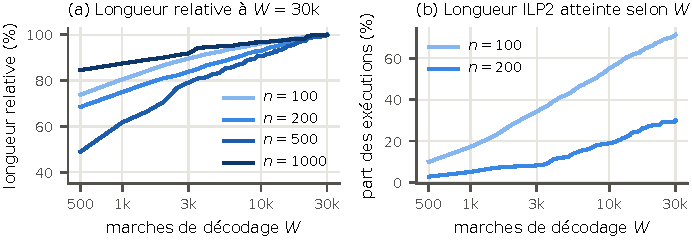
\includegraphics[width=\textwidth]{fig4_budget.pdf}
\caption{Effet du nombre de marches de décodage $W$. (a) Longueur moyenne des chemins, relative à la longueur obtenue avec $W=30\,000$. (b) Part des exécutions qui atteignent la longueur ILP2 (instances disposant d'une solution ILP2).}
\label{fig:budget}
\end{figure}

\subsection{Discussion et limites}

Les résultats confirment l'intérêt de combiner des composants appris et exacts. L'anticipation fournit au décodeur une information exacte, peu coûteuse à calculer sur un DAG, au lieu de demander au modèle d'embeddings de l'apprendre. $G$ sert au guidage et à la vérification finale plutôt qu'à l'objectif d'apprentissage des embeddings, ce qui recentre l'apprentissage sur l'ordre du chemin, tandis que l'étape d'extraction garantit la réalisabilité.

La méthode a des limites claires. C'est une heuristique, qui ne doit pas remplacer ILP2 lorsque l'optimalité doit être garantie. Son écart à ILP2 croît avec $n$ à budget fixé, et sur de petites voies réelles l'énumération exacte est à la fois exacte et plus rapide. Les embeddings sont entraînés pour chaque instance, ce qui ajoute un coût d'entraînement qu'un modèle entraîné sur plusieurs instances éviterait. Enfin, notre évaluation sur données réelles ne couvre que de petites voies, et l'orientation des réactions réversibles est une simplification.

% ============================================================
\section{Conclusion}
% ============================================================

Nous avons présenté Skew-GRAM, qui applique le modèle Skip-Gram du TAL au problème One-to-one SkewGRAM issu de la biologie : trouver un plus long chemin dans un DAG dont les sommets sont connexes dans un second graphe. Des embeddings appris à partir de marches aléatoires orientées guident un décodeur Monte-Carlo, avec une anticipation exacte sur le DAG et un bonus de connexité, et une étape exacte d'Union-Find rend tout chemin renvoyé réalisable. Sur 368 instances synthétiques disposant d'une solution ILP2, la méthode atteint la longueur ILP2 dans la plupart des exécutions à 100 sommets et s'exécute bien plus vite qu'ILP2, avec une accélération qui croît avec la taille des graphes ; ses résultats moyens varient peu d'une graine à l'autre, elle trouve l'optimum exact sur 25 voies métaboliques réelles, et elle passe à l'échelle de graphes de 1000 sommets. Nos travaux futurs porteront sur des réseaux réels plus grands, un décodeur plus rapide (marches en parallèle, bonus $G$ incrémental, budget adaptatif) et des embeddings entraînés sur plusieurs instances.

% ============================================================
% RÉFÉRENCES (style splncs04)
% ============================================================

\begin{thebibliography}{10}

\bibitem{sidi2022}
Ahmed Sidi, M.L., Bocquillon, R., Mohamed Babou, H., Dhib, C., Néron, E., Soukhal, A., Nanne, M.F.: Improved approaches to solve the one-to-one SkewGraM problem. Computers \& Operations Research \textbf{138}, 105584 (2022)

\bibitem{sidi_dl}
Ahmed Sidi, M.L., Mohamed Babou, H., Dhib, C.: Deep learning approaches for finding a longest DG-consistent path in biological networks. Preprint (2024)

\bibitem{sidi}
Ahmed Sidi, M.L., Mohamed Babou, H., Dhib, C., Néron, E., Soukhal, A., Nanne, M.F.: Constraint programming approaches for finding conserved metabolic and genomic patterns. Computers \& Operations Research \textbf{183}, 107166 (2025)

\bibitem{bellman1958}
Bellman, R.: On a routing problem. Quarterly of Applied Mathematics \textbf{16}(1), 87--90 (1958)

\bibitem{bello2016}
Bello, I., Pham, H., Le, Q.V., Norouzi, M., Bengio, S.: Neural combinatorial optimization with reinforcement learning. arXiv preprint arXiv:1611.09940 (2016)

\bibitem{dai2017}
Dai, H., Khalil, E.B., Zhang, Y., Dilkina, B., Song, L.: Learning combinatorial optimization algorithms over graphs. In: Advances in Neural Information Processing Systems, vol.~30 (2017)

\bibitem{erdos1959}
Erd\H{o}s, P., Rényi, A.: On random graphs I. Publicationes Mathematicae Debrecen \textbf{6}, 290--297 (1959)

\bibitem{fertin2012}
Fertin, G., Mohamed Babou, H., Rusu, I.: Algorithms for subnetwork mining in heterogeneous networks. In: Experimental Algorithms (SEA 2012). LNCS, vol.~7276, pp. 184--194. Springer (2012)

\bibitem{grover}
Grover, A., Leskovec, J.: node2vec: scalable feature learning for networks. In: Proceedings of the 22nd ACM SIGKDD International Conference on Knowledge Discovery and Data Mining, pp. 855--864 (2016)

\bibitem{kanehisa2000}
Kanehisa, M., Goto, S.: KEGG: Kyoto Encyclopedia of Genes and Genomes. Nucleic Acids Research \textbf{28}(1), 27--30 (2000)

\bibitem{karalias2020}
Karalias, N., Loukas, A.: Erd\H{o}s goes neural: an unsupervised learning framework for combinatorial optimization on graphs. In: Advances in Neural Information Processing Systems, vol.~33 (2020)

\bibitem{kingma2014}
Kingma, D.P., Ba, J.: Adam: a method for stochastic optimization. arXiv preprint arXiv:1412.6980 (2014)

\bibitem{mikolov}
Mikolov, T., Sutskever, I., Chen, K., Corrado, G., Dean, J.: Distributed representations of words and phrases and their compositionality. In: Advances in Neural Information Processing Systems, vol.~26 (2013)

\bibitem{perozzi}
Perozzi, B., Al-Rfou, R., Skiena, S.: DeepWalk: online learning of social representations. In: Proceedings of the 20th ACM SIGKDD International Conference on Knowledge Discovery and Data Mining, pp. 701--710 (2014)

\bibitem{sharan2006}
Sharan, R., Ideker, T.: Modeling cellular machinery through biological network comparison. Nature Biotechnology \textbf{24}(4), 427--433 (2006)

\bibitem{tarjan1975}
Tarjan, R.E.: Efficiency of a good but not linear set union algorithm. Journal of the ACM \textbf{22}(2), 215--225 (1975)

\bibitem{vinyals2015}
Vinyals, O., Fortunato, M., Jaitly, N.: Pointer networks. In: Advances in Neural Information Processing Systems, vol.~28 (2015)

\bibitem{zaharia}
Zaharia, A., Labedan, B., Froidevaux, C., Denise, A.: CoMetGeNe: mining conserved neighborhood patterns in metabolic and genomic contexts. BMC Bioinformatics \textbf{20}, 19 (2019)

\end{thebibliography}

\end{document}
